% -*- eval: (auto-fill-mode 1); fill-column: 80; -*-

\documentclass[11pt]{asaproc}

\usepackage{graphicx}
\usepackage{natbib}
\usepackage[hyphens]{url}
\usepackage{color}
\usepackage{times}
\usepackage{verbatim}
\usepackage{amsmath}
%\usepackage{enumitem}
\usepackage[hidelinks,breaklinks=true]{hyperref}
\usepackage{float}
\usepackage{caption}
\usepackage{subcaption}

\renewcommand\labelenumi{(\roman{enumi})}
\renewcommand\theenumi\labelenumi

\title{semicircledistr: An R Package to Simulate the Semicircle Distribution}

\author{Marcus Quincy \thanks{College of Science, Utah State University, Logan, UT 84322--3900, USA.
    E-mail: \url{mswr@marcusquincy.org}}
  \and Dylan Perrenoud \thanks{Department of Mathematics and Statistics, Utah State University, Logan, UT 84322--3900, USA.
    E-mail: \url{dylan.perrenoud@usu.edu}}
  \and Matthew White \thanks{Department of Mathematics and Statistics, Utah State University, Logan, UT 84322--3900, USA.
    E-mail: \url{m.white@usu.edu}}
}

\begin{document}

\renewcommand{\topfraction}{1.0}
\renewcommand{\bottomfraction}{1.0}
\renewcommand{\textfraction}{0.0}
\renewcommand{\floatpagefraction}{1.0}
\renewcommand{\dbltopfraction}{1.0}


\maketitle

\begin{abstract}
This paper introduces semicircledistr, an R package designed to simulate and analyze the Wigner semicircle distribution, a fundamental concept in random matrix theory. Despite its theoretical importance, the distribution—defined by a semicircular density over a bounded interval—has no native implementation on CRAN. The package offers essential distribution functions, including the density, cumulative distribution, quantile, and random sampling. Its implementation is validated through simulations of large symmetric random matrices, illustrating Wigner’s semicircle law, and through the convergence behavior of a transformed beta distribution.
\end{abstract}

\begin{keywords}Semicircle distribution; CRAN; R Package; Software; Random matrix; Simulation
\end{keywords}


%%%%%%%%%%%%%%%%%%%%%%%%%
\section{Introduction}
\label{Introduction}
%%%%%%%%%%%%%%%%%%%%%%%%%

The semicircle distribution was first proposed by physicist Eugene Wigner who
observed the semicircle law for certain classes of random matrices arising in
quantum mechanical investigations \citep{wigner1955characteristic}. It is called the Wigner semicircle
distribution because the probability density function forms a symmetrical
semicircle shape with an area of 1. The parameters of this distribution are
the radius \textit{R} and an offset parameter, which is a linear shift along the
x-axis (by default, the distribution is centered at $X = 0$). The semicircle
distribution is a continuous univariate distribution which only has a non-zero
probability within its radius.

% citation for above: Weisstein, Eric W. "Wigner's Semicircle Law." From MathWorld--A Wolfram Web Resource. https://mathworld.wolfram.com/WignersSemicircleLaw.html
% citation for wigner's first paper: Wigner, E. "Characteristic Vectors of Bordered Matrices with Infinite Dimensions." Ann. of Math. 62, 548-564, 1955.

The Wigner Semicircle distribution has application in the realm of random
matrices. Given an $N \times N$ symmetric random matrix in which all values are independent and
identically distributed (i.i.d.), the eigenvalues of such a matrix will converge
to the semicircle distribution as \textit{N} approaches infinity. This applies
regardless of the probability distribution, so long as the values are randomly
sampled and are independent. For some distributions such as the uniform
distribution, the eigenvalues of the i.i.d. matrix will contain exactly one large
value, and the remaining eigenvalues will converge to the semicircle
distribution \citep{weisstein2025wigner}.

Currently, there does not exist an implementation of the Wigner Semicircle
distribution on the Comprehensive R Archive Network (CRAN), and we were unable to find any R implementation of such a
package. Therefore, the contribution of this project is to create an R
implementation of the standard R distribution functions for the Wigner
semicircle distribution. This R package will follow existing conventions of
including functions for the probability density function, cumulative
distribution function, quantile function, and random generation function.

In addition to providing an implementation of the Wigner semicircle
distribution, we provide examples of its usage and demonstrate that random
matrices do converge to the distribution. Finally, we show that for a beta
distribution in the special case $\alpha = \beta = \frac{3}{2}$, random
variables converge to the semicircle distribution \citep{wikimedia_wigner}. This relationship
between the beta distribution and the semicircle distribution makes it easier to
compute some statistical quantiles for the Wigner distribution in terms of the
beta distribution, which is better known.

%%%%%%%%%%%%%%%%%%%%%%%%%
\section{The R Package}
\label{Package}
%%%%%%%%%%%%%%%%%%%%%%%%%

The repository for the R package can be found at \url{https://github.com/matthewwhite1/semicircledistr}.
%%% The four functions

\subsection{Probability Density Function}

The probability density function (PDF) of a distribution is a function whose
value is the relative probability that the value of a random variable from the
distribution is equal to that sample. The PDF of the semicircle distribution can
be computed using the following closed-form solution in $[-R+a, R+a]$:

\begin{equation}
  f(x) = \frac{2}{\pi R^2}\sqrt{R^2-(x-a)^2}
\end{equation}

Outside of that range, $f(x) = 0$ \citep{wikimedia_wigner}.

In R packages, It is convention that this function is prefixed with \textit{d},
such as the \texttt{dnorm} function corresponding to the normal distribution. As
such, we created a \texttt{dsemicircle} function which is the PDF for the Wigner
Semicircle distribution.

The \texttt{dsemicircle} function takes 3 arguments: \texttt{x} which is a
vector of values to calculate the probability density of, \texttt{R} which is
the radius of the circle, and \texttt{a} which is an optional parameter which
offsets the distribution on the X axis (by default it is centered at 0). The
function makes sure to perform validation on the inputs, such as ensuring that
the inputs are numeric values. All the components of the closed form solution of
this are provided in base R, making the implementation of the PDF
straightforward.

The distribution has a mean, median, and mode at \textit{a}, and has a variance of
$\frac{R^2}{4}$.


\subsection{Cumulative Distribution Function}

The cumulative distribution function of a distribution describes the probability
that a value is less than or equal to \textit{x} in a distribution. The CDF of
the Wigner semicircle distribution is given using a closed form solution, which
is defined from $[-R+a, R+a]$.

\begin{equation}
  F(x) = \frac{1}{2} + \frac{(x-a)\sqrt{R^2-(x-a)^2}}{\pi R^2} +
  \frac{sin^{-1}(\frac{x-a}{R})}{\pi}
\end{equation}

Following conventions of existing R packages, the function computing the CDF of
the Wigner semicircle distribution is called \texttt{psemicircle}. This function
takes the same arguments as \texttt{dsemicircle}, that is \texttt{x} which is a
vector of values to calculate the cumulative probability of, \texttt{R} which is
the radius of the circle, and \texttt{a} which is the optional offset parameter.
Furthermore, validation is performed to ensure function inputs are valid. Just
like the PDF, the closed form solution of the CDF can be implemented in R.


\subsection{Quantile Function}

The quantile function (also known as the inverse cumulative distribution function)
returns the value $x$ such that the cumulative distribution function (CDF) evaluated at $x$
equals a given probability $p$. That is, for a given $p \in [0,1]$, the quantile function
solves for $x$ in the equation:

\[
F(x) = p
\]

For the Wigner semicircle distribution, the CDF $F(x)$ involves both a square root and an inverse sine function. While it is possible to write down the CDF in closed form, these components make it unable to algebraically solve for $x$ in terms of $p$. As a result, the inverse CDF (i.e., the quantile function) does not have a closed-form solution.

To compute quantiles numerically, we use the \texttt{uniroot} function from base R. This function performs numerical root-finding to solve equations of the form $f(x) = 0$ for a single variable $x$. In the context of the \texttt{qsemicircle} function, \texttt{uniroot} is used to find the value of $x$ such that:

\[
F(x) - p = 0
\]

This process is performed over the domain $[a - R, a + R]$, the support of the Wigner semicircle distribution. The \texttt{uniroot} function is used to iteratively narrow the interval containing the root, guaranteeing convergence as long as the function is continuous and changes sign within the interval.

The \texttt{qsemicircle} function accepts \texttt{p}, a numeric vector of probabilities between 0 and 1; \texttt{R}, the radius of the semicircle; and \texttt{a}, an optional numeric parameter that shifts the distribution along the x-axis (defaulting to 0).

Basic input validation is included to ensure that values of \texttt{p} lie within $[0, 1]$, \texttt{R} is positive, and \texttt{a} is numeric. For edge cases where $p = 0$ or $p = 1$, the function returns $a - R$ or $a + R$, respectively. For all other values, \texttt{uniroot} is called internally, using the previously defined \texttt{psemicircle} function to find the value of $x$ corresponding to the given probability $p$.

This numerical approach ensures an accurate quantile computation even in the absence of a closed-form inverse function.

\subsection{Random Sampling}

Random sampling from a probability distribution is a common technique in simulation and probabilistic modeling. For the Wigner semicircle distribution, random samples can be generated using the inverse transform sampling method. This method relies on the fact that if $U$ is a uniform random variable on $[0, 1]$, then $X = F^{-1}(U)$ has the desired distribution, where $F^{-1}$ is the quantile function.

In this package, the random sampling function is called \texttt{rsemicircle}, again following standard R naming conventions. It uses the quantile function defined in \texttt{qsemicircle} to transform uniform samples into semicircle-distributed values.

The \texttt{rsemicircle} function also takes three arguments. The first argument, \texttt{n}, is an integer indicating the number of random samples to generate. The second argument, \texttt{R}, is the radius of the semicircle and must be a positive number. The third argument, \texttt{a}, is the optional numeric parameter that offsets the distribution on the x-axis (with a default value of 0).

The function first checks that the inputs are valid: \texttt{n} must be an integer, \texttt{R} must be positive, and \texttt{a} must be numeric. Then, it generates \texttt{n} independent values from the uniform distribution on $[0, 1]$ using \texttt{stats::runif(n)}. These uniform values are then passed to \texttt{qsemicircle}, which transforms them into random samples from the Wigner semicircle distribution leveraging the previously implemented quantile function.





%%%%%%%%%%%%%%%%%%%%%%%%%
\section{Applying Package Functions}
\label{Application}
%%%%%%%%%%%%%%%%%%%%%%%%%

\subsection{Verifying Wigner's Semicircle Law}

Recalling from earlier in this paper: The distribution of the eigenvalues of an $N \times N$ symmetric random matrix will converge to the semicircle distribution as $N$ goes to infinity.

In order to verify this law using the functions in our package, we can perform the following steps:
\begin{enumerate}
    \item Simulate three Gaussian random matrices with different sizes ($1000 \times 1000$, $2500 \times 2500$, and $5000 \times 5000$) \citep{jiang2021wigner}
    \item Symmetrize and scale each matrix, which is performed by adding the original matrix's transpose to itself and dividing by $\sqrt{2N}$
    \item Compute the eigenvalues of each matrix
    \item Plot histograms to investigate the distributions
\end{enumerate}

\begin{figure}[H]
    \centering
    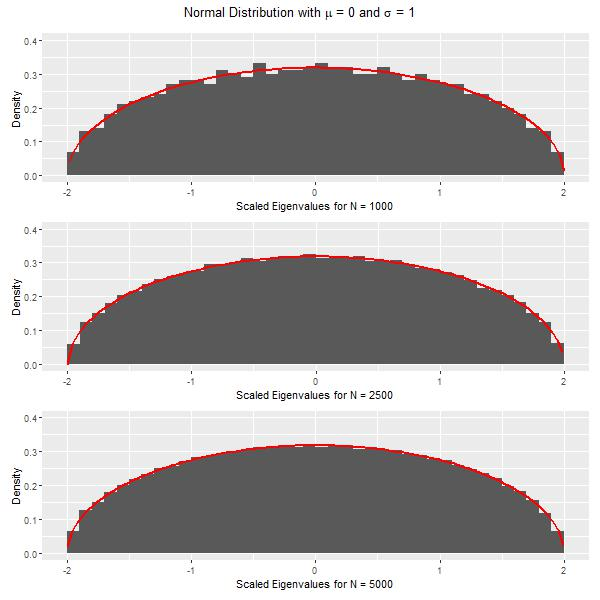
\includegraphics[scale=0.38]{figures/SemiLaw.jpeg}
    \caption{Verification of Wigner's Semicircle Law on normal random matrices}
    \label{fig:semilaw}
\end{figure}

Figure \ref{fig:semilaw} shows the results of following these steps. We can see that as $N$ increases, the distribution more closely follows the red semicircle curve, which is created from our \texttt{dsemicircle} function.

While the normal distribution was the first distribution we looked at, it is not the only probability distribution that Wigner's semicircle law applies to. We also applied the same steps to the exponential distribution, the uniform distribution, and our own implementation of the semicircle distribution.

For the semicircle to cleanly be between -2 and 2, the random matrix has to have a mean of 0 and a variance of 1. This required different scaling depending on the distribution - these different scaling techniques can be seen in the "Scripts" folder of the R package repository.

\begin{figure}[H]
    \centering
    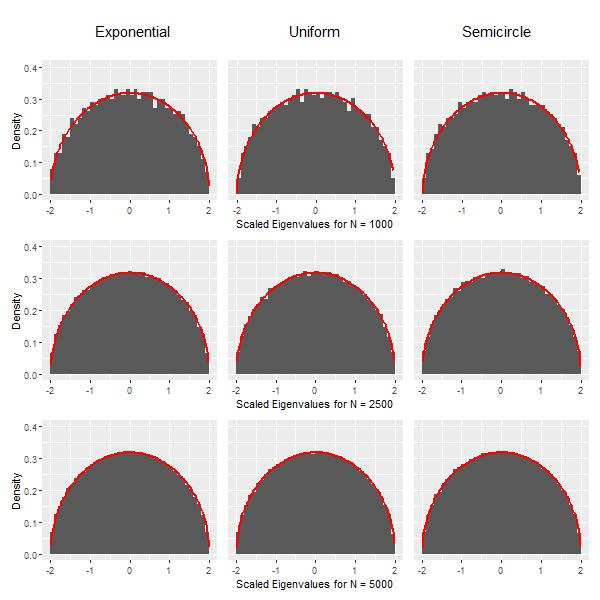
\includegraphics[width=10cm,height=8cm]{figures/SemiLaw_Combined.jpeg}
    \caption{Verification of Wigner's Semicircle Law on random matrices. The left column comes from an exponential distribution with $\lambda=1$. The middle column comes from a uniform distribution with $a=-\sqrt{3}$ and $b=\sqrt{3}$. The right column comes from our own implementation of the semicircle distribution with $R=2$ and $a=0$.}
    \label{fig:semilaw_combined}
\end{figure}

Figure \ref{fig:semilaw_combined} shows that Wigner's semicircle law applies to the exponential distribution, the uniform distribution, and even the semicircle distribution.

\subsection{Verifying a Beta Transformation Theory}

As referenced earlier in this paper: If $Y$ is a beta-distributed random variables with parameters $\alpha = \beta = \frac{3}{2}$, then the random variable $2RY-R$ exhibits a Wigner semicircle distribution with radius R.

In order to verify this theorem using the functions in our package, we can perform the following steps:
\begin{enumerate}
    \item Simulate three random vectors from a beta distribution with parameters $\alpha = \beta = \frac{3}{2}$ and different sizes (1000, 10000, 100000)
    \item Calculate a transformation of each of these vectors given $2RY-R$, choosing a radius value of 2
    \item Examine the distributions
\end{enumerate}

\begin{figure}[H]
     \centering
     \begin{subfigure}[b]{0.4\textwidth}
         \centering
         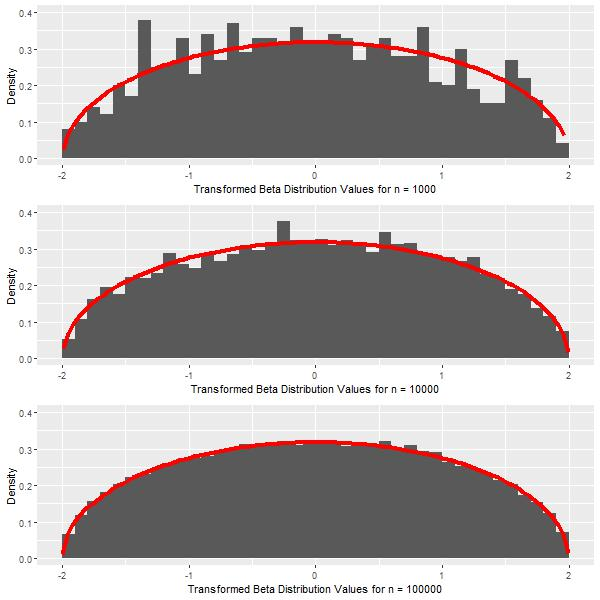
\includegraphics[width=\textwidth]{figures/BetaTrans.jpeg}
         \caption{Histograms}
         \label{fig:betatrans_hist}
     \end{subfigure}
     \hfill
     \begin{subfigure}[b]{0.4\textwidth}
         \centering
         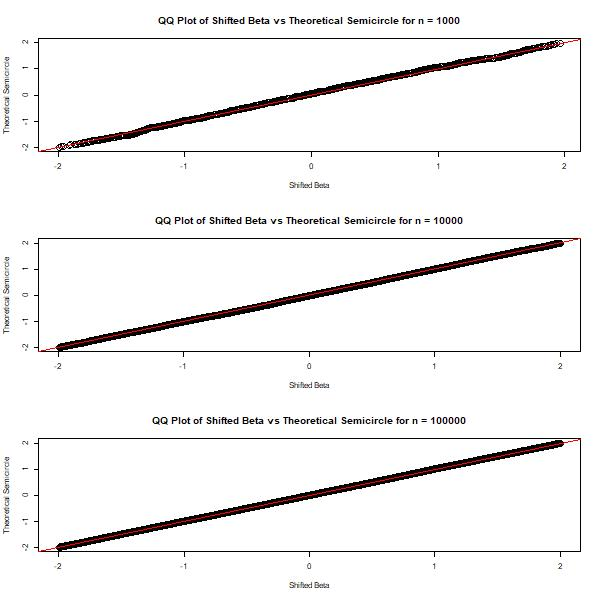
\includegraphics[width=\textwidth]{figures/BetaTrans_QQ.jpeg}
         \caption{QQ Plots}
         \label{fig:betatrans_qq}
     \end{subfigure}
        \caption{Verification of a beta transformation theory}
        \label{fig:betatrans}
\end{figure}

Figure \ref{fig:betatrans} shows that this theorem seems to hold when compared to the theoretically based functions in our package. The histograms show that the distribution looks more like a semicircle as the size of the vector increases, and the QQ plots corroborate this message.


%%%%%%%%%%%%%%%%%%%%%%%%%
\section{Conclusions and Future Work}
\label{Conclusion}
%%%%%%%%%%%%%%%%%%%%%%%%%

This report detailed the R package that was created to simulate the semicircle distribution, which does not have any other current R packages that simulate it. This R package includes the four probability distribution simulation functions, documentation for these functions, a README, and unit tests. We were able to apply our functions to simulated data to determine that both our functions work properly and that the Wigner semicircle law seems to hold.

If we had more time to work on this project, we would have liked to do some more advanced math with the distribution simulation. For example, the Wikipedia page for the Wigner semicircle distribution provides some details about the special properties of the moments of this distribution when $R=2$ \citep{wikimedia_wigner}.

Starting in May 2025, we will work on submitting our package to CRAN for public use. Before doing this, we still need to refine our DESCRIPTION file and select an official package maintainer. Fortunately, we have already accomplished most of the necessary tasks for submitting an R package to CRAN. Hopefully, other people can find some meaning in using our package to study ideas like Wigner's semicircle law.


\bibliographystyle{apalike}

%\bibliographystyle{elsarticle-harv}
% modified to add
%     \itemsep=0pt
% to 2nd line of file paper.bbl

{\footnotesize
\bibliography{references}}

\appendix
\section{R Package Code}

\begin{verbatim}
dsemicircle <- function(x, R, a = 0) {
  if (!is.numeric(x)) {
    stop("x must be numeric.")
  }
  if (R <= 0) {
    stop("R must be positive.")
  }
  if (!is.numeric(a)) {
    stop("a must be numeric.")
  }
  ifelse(abs(x - a) > R, 0, (2 / (pi * R^2)) * sqrt(R^2 - (x - a)^2))
}


psemicircle <- function(x, R, a = 0) {
  if (!is.numeric(x)) {
    stop("x must be numeric.")
  }
  if (R <= 0) {
    stop("R must be positive.")
  }
  if (!is.numeric(a)) {
    stop("a must be numeric.")
  }
  result <- numeric(length(x))
  for (i in 1:length(x)) {
    val <- x[i] - a
    if (abs(val) > R) {
      stop("x must be within radius.")
    }
    result[i] <- 0.5 + (val * sqrt(R^2 - val^2)) 
    / (pi * R^2) + asin(val / R) / pi
  }
  return(result)
}


qsemicircle <- function(p, R, a = 0) {
  if (!is.numeric(p) || any(p < 0) || any(p > 1)) {
    stop("p must be between 0 and 1.")
  }
  if (R <= 0) {
    stop("R must be positive.")
  }
  if (!is.numeric(a)) {
    stop("a must be numeric.")
  }
  quantile_fn <- function(prob) {
    sapply(prob, function(p) {
      if (p == 0) return(a - R)
      if (p == 1) return(a + R)
      uniroot(function(x) psemicircle(x, R, a) - p,
              lower = a - R, upper = a + R)$root
    })
  }
  quantile_fn(p)
}


rsemicircle <- function(n, R, a = 0) {
  if (!is.numeric(n) || n != round(n)) {
    stop("n must be an integer.")
  }
  if (R <= 0) {
    stop("R must be positive.")
  }
  if (!is.numeric(a)) {
    stop("a must be numeric.")
  }
  u <- stats::runif(n)
  qsemicircle(u, R, a)
}


library(ggplot2)
library(pracma) # for random matrices
library(patchwork)


# Create 3 N by N random matrices
# Stopping at 5000 instead of 10000 to save on computation time
set.seed(1234)

norm_1000 <- randn(1000)
norm_1000_sym <- (norm_1000 + t(norm_1000)) / sqrt(2 * 1000)
ev_1000 <- eigen(norm_1000_sym)
ev_1000_df <- data.frame(ev = ev_1000$values)

norm_2500 <- randn(2500)
norm_2500_sym <- (norm_2500 + t(norm_2500)) / sqrt(2 * 2500)
ev_2500 <- eigen(norm_2500_sym)
ev_2500_df <- data.frame(ev = ev_2500$values)

norm_5000 <- randn(5000)
norm_5000_sym <- (norm_5000 + t(norm_5000)) / sqrt(2 * 5000)
ev_5000 <- eigen(norm_5000_sym) # This takes a few minutes to run
ev_5000_df <- data.frame(ev = ev_5000$values)

# Create histograms
g1 <- ggplot(ev_1000_df, aes(ev)) +
  geom_histogram(aes(y = after_stat(density)), 
  breaks = seq(-2, 2, by = 0.1)) + xlab("Scaled Eigenvalues for N = 1000")

g2 <- ggplot(ev_2500_df, aes(ev)) +
  geom_histogram(aes(y = after_stat(density)), 
  breaks = seq(-2, 2, by = 0.1)) +
  xlab("Scaled Eigenvalues for N = 2500")

g3 <- ggplot(ev_5000_df, aes(ev)) +
  geom_histogram(aes(y = after_stat(density)), 
  breaks = seq(-2, 2, by = 0.1)) +
  xlab("Scaled Eigenvalues for N = 5000")

jpeg("Plots/SemiLaw_NoCurve.jpeg", width = 600, height = 600)

g1 /
  g2 /
  g3 + plot_annotation(
    title = expression(paste("Normal Distribution with ", 
    mu, " = 0 and ", sigma, " = 1")),
    theme = theme(plot.title = element_text(hjust = 0.5))
  ) &
  scale_y_continuous("Density",
    breaks = seq(0, 0.4, by = 0.1),
    limits = c(0, 0.4)
  )

dev.off()


# Add semicircle distribution densities
g1 <- g1 +
  stat_function(fun = dsemicircle, args = list(R = 2), 
  lwd = 1, color = "red")

g2 <- g2 +
  stat_function(fun = dsemicircle, args = list(R = 2), 
  lwd = 1, color = "red")

g3 <- g3 +
  stat_function(fun = dsemicircle, args = list(R = 2), 
  lwd = 1, color = "red")

jpeg("Plots/SemiLaw.jpeg", width = 600, height = 600)

g1 /
  g2 /
  g3 + plot_annotation(
    title = expression(paste("Normal Distribution with ", mu, " = 0 
    and ", sigma, " = 1")),
    theme = theme(plot.title = element_text(hjust = 0.5))
  ) &
  scale_y_continuous("Density",
                     breaks = seq(0, 0.4, by = 0.1),
                     limits = c(0, 0.4)
  )

dev.off()


library(ggplot2)
library(gridExtra)


# Create random variable transformations
set.seed(1234)

R <- 2

# n = 1000
Y1 <- rbeta(1000, (3 / 2), (3 / 2))
U1 <- 2 * R * Y1 - R
U1_df <- data.frame(U1_vals = U1)

# n = 10000
Y2 <- rbeta(10000, (3 / 2), (3 / 2))
U2 <- 2 * R * Y2 - R
U2_df <- data.frame(U2_vals = U2)

# n = 100000
Y3 <- rbeta(100000, (3 / 2), (3 / 2))
U3 <- 2 * R * Y3 - R
U3_df <- data.frame(U3_vals = U3)

# Create histograms
g1 <- ggplot(U1_df, aes(U1_vals)) +
  geom_histogram(aes(y = after_stat(density)), 
  breaks = seq(-2, 2, by = 0.1)) +
  scale_y_continuous("Density", breaks = seq(0, 0.4, by = 0.1), 
  limits = c(0, 0.4)) +
  xlab("Transformed Beta Distribution Values for n = 1000")

g2 <- ggplot(U2_df, aes(U2_vals)) +
  geom_histogram(aes(y = after_stat(density)), 
  breaks = seq(-2, 2, by = 0.1)) +
  scale_y_continuous("Density", breaks = seq(0, 0.4, by = 0.1), 
  limits = c(0, 0.4)) +
  xlab("Transformed Beta Distribution Values for n = 10000")

g3 <- ggplot(U3_df, aes(U3_vals)) +
  geom_histogram(aes(y = after_stat(density)), 
  breaks = seq(-2, 2, by = 0.1)) +
  scale_y_continuous("Density", breaks = seq(0, 0.4, by = 0.1), 
  limits = c(0, 0.4)) +
  xlab("Transformed Beta Distribution Values for n = 100000")

jpeg("Plots/BetaTrans_NoCurve.jpeg", width = 600, height = 600)

grid.arrange(g1, g2, g3)

dev.off()

# Add semicircle distribution densities
g1 <- g1 +
  stat_function(fun = dsemicircle, args = R, lwd = 1.5, color = "red")

g2 <- g2 +
  stat_function(fun = dsemicircle, args = R, lwd = 1.5, color = "red")

g3 <- g3 +
  stat_function(fun = dsemicircle, args = R, lwd = 1.5, color = "red")

jpeg("Plots/BetaTrans.jpeg", width = 600, height = 600)

grid.arrange(g1, g2, g3)

dev.off()

jpeg("Plots/BetaTrans_QQ.jpeg", width = 600, height = 600)

# Check with a QQ plot
par(mfrow = c(3, 1))

theoretical1 <- qsemicircle(ppoints(1000), R)
qqplot(U1, theoretical1, 
        main = "QQ Plot of Shifted Beta vs 
        Theoretical Semicircle for n = 1000",
       xlab = "Shifted Beta", ylab = "Theoretical Semicircle", cex = 2)
abline(a = 0, b = 1, col = "red")

theoretical2 <- qsemicircle(ppoints(10000), R)
qqplot(U2, theoretical2, 
        main = "QQ Plot of Shifted Beta vs 
        Theoretical Semicircle for n = 10000",
       xlab = "Shifted Beta", ylab = "Theoretical Semicircle", cex = 2)
abline(a = 0, b = 1, col = "red")

theoretical3 <- qsemicircle(ppoints(100000), R)
qqplot(U3, theoretical3, 
        main = "QQ Plot of Shifted Beta vs 
        Theoretical Semicircle for n = 100000",
       xlab = "Shifted Beta", ylab = "Theoretical Semicircle", cex = 2)
abline(a = 0, b = 1, col = "red")

dev.off()

\end{verbatim}


\end{document}

